% % \begin{figure}
% % 	\centering
% 	\begin{minipage}{.5\textwidth}
% 		\centering
% 		\includegraphics[keepaspectratio]{Imagenes/exp1/biseccion_f.pdf}
% 		\captionof{figure}{A figure}
% 		\label{fig:test1}
% 	\end{minipage}%
% 	\begin{minipage}{.5\textwidth}
% 		\centering
% 		\includegraphics[keepaspectratio]{Imagenes/exp1/biseccion_f.pdf}
% 		\captionof{figure}{Another figure}
% 		\label{fig:test2}
% 	\end{minipage}
% \end{figure}

\subsection{Primeras experimentaciones}

\begin{figure}[!h]
	\begin{center}
		  \includegraphics[keepaspectratio]{../Imagenes/exp1/biseccion_f.pdf}
		  \caption{Bisección\_f para $\alpha=4.0, \epsilon = 10^{-6}, criterio = 1\  con \ max\_iter=20$}
		  \label{fig:contra1}
	\end{center}
\end{figure}
\FloatBarrier
~

\begin{figure}[!h]
	\begin{center}
		  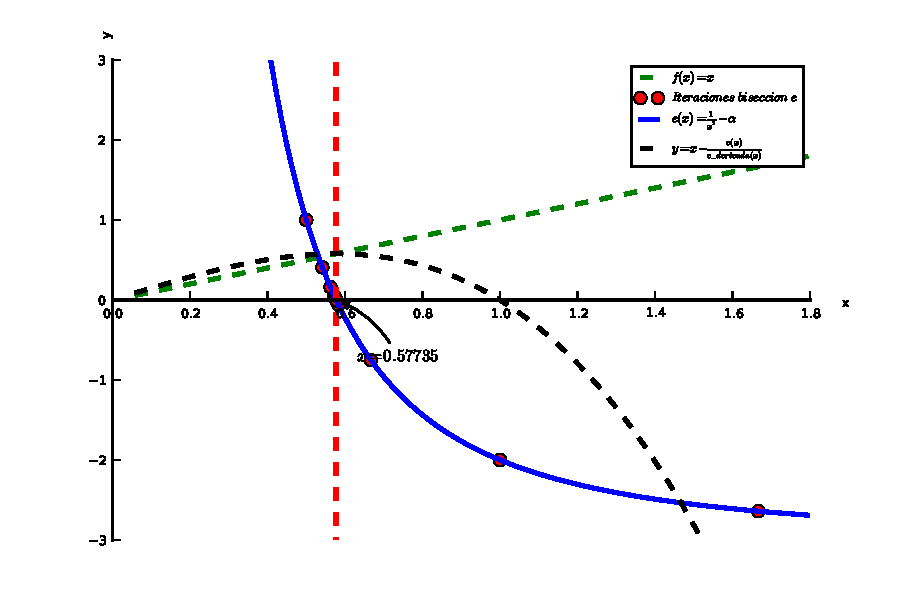
\includegraphics[keepaspectratio]{../Imagenes/exp1/biseccion_e.pdf}
		  \caption{Bisección\_e para $\alpha=6.0, \epsilon = 10^{-6}, criterio = 3$}
		  \label{fig:contra1}
	\end{center}
\end{figure}
\FloatBarrier
Los resultados tanto para $biseccion\_f$ como para $biseccion\_e$ fueron los esperados. Los métodos convergen al resultado para cualquier valor de $\alpha$ (Fueron evaluados valores entre 0 y 10000 aproximadamente,
con bastante granularidad). Para realizar los gráficos fueron elegidos los valores de $\alpha$ 4.0 para $f$ y 6.0 para $e$ únicamente debido a que permiten utilizar una escala que nos deja apreciar los aspectos
relevantes del análisis. Los puntos rojos corresponden al valor de $x$ en cada iteración del método. Con el correr de las iteradas, los puntos van amontonándose alrededor de la raíz teórica de la función.

Un aspecto llamativo de los resultados obtenidos en esta etapa es el hecho de que 
a medida que los valores de $\alpha$ crecen, bisección\_e requiere de una mayor cantidad de iteraciones (en comparación con $f$) para obtener un valor cercano a la raíz de la función. Por ejemplo,
tomando 40 iteraciones en cada experimento y variando el valor de alfa, obtuvimos que: 

Para $\alpha = 0.1$, $f(x\_40) \approx 1*10^{-13}$ y $e(x\_40) \approx 1*10^{-13}$. 

Para $\alpha = 7.0$ : 
$f(x\_40) \approx 1*10^{-11}$ y $e(x\_40) \approx 1*10^{-10}$. 

Y ya para $\alpha = 10000.0$: $f(x\_40) \approx 1*10^{-5}$ y $e(x\_40) \approx 0.01$

Notemos que estamos utilizando el criterio (3) para analizar la calidad de la solución obtenida.

Por lo general biseccion\_e se comprta peor que biseccion\_f (Terminar de pensar por qué)

Contrariamente a lo que suponíamos, al analizar newton\_f \ descubrimos que, luego de fijar $\alpha$ (distinto de cero), el método converge para cualquier semilla inicial que tomemos (también distinta de 0).
Pensemos un poco por qué sucede esto: 
Anteriormente ya demostramos que si $seed\_inicial > \sqrt{\alpha}$ entonces el método converge (ejercicio 3 de la práctica). 
Sin embargo, ¿ qué sucede cuando pertenece al itervalo $(0,\sqrt{\alpha})$. $x_1$ es el valor 
obtenido a partir de la interesección entre la recta tangente a $f(x)$ en $(x_0,f(x_0)$ y el eje de abscisas. Experimentalmente parecería ser que el valor de $x_1$ obtenido luego de la primera 
iteración es mayor a $\sqrt{\alpha}$. Este hecho puede explicarse en función la pendiente de la recta tangente en la semilla inicial. Como la misma tiene un valor peque\~no en módulo pero positivo
(menor a $2*\sqrt{\alpha}$), no es ilógico pensar que cortará al eje de abscisas en un valor de $x$ mayor a  $\sqrt{\alpha}$. El siguiente gráfico intenta representar esta idea:  

\begin{figure}[!h]
	\begin{center}
		  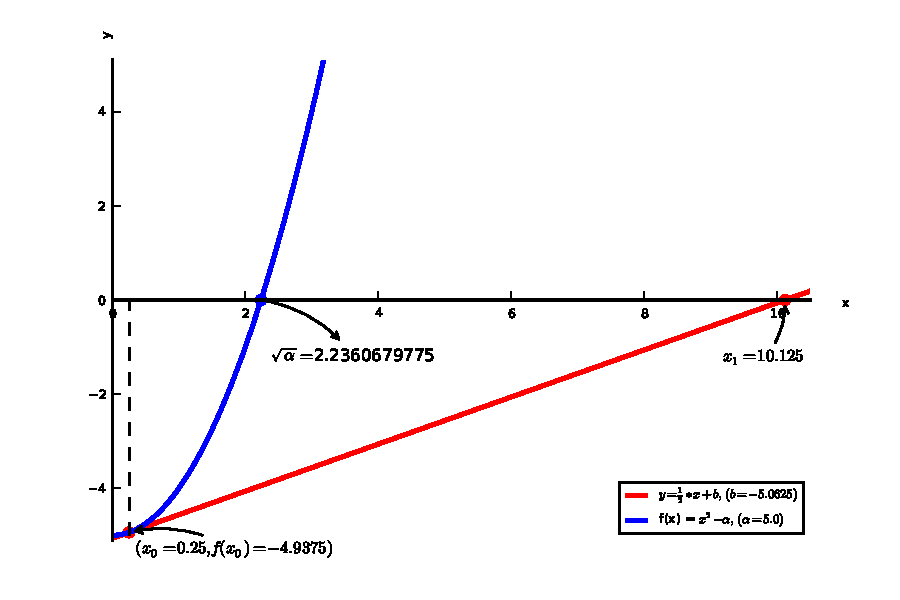
\includegraphics[keepaspectratio]{../Imagenes/exp1/recta_tangente.pdf}
		  \caption{Recta tangente a la curva con $x_0=0.25$ y $\alpha=5.0$}
		  \label{fig:contra1}
	\end{center}
\end{figure}
\FloatBarrier

Nótese que en los casos en donde $x_0$ comienza con valores peque\~nos en módulo obtenemos a partir de la primera iteración un $x\_1 >> \sqrt{\alpha}$. A medida que nos fuimos
acercando por izquierda, para valores en donde $x_{0} \approx \sqrt{\alpha}$,
experimentalmente también obtuvimos que $x\_1 > \sqrt{\alpha}$, lo cual explica el hecho de que newton\_f converja para cualquier semilla inicial.

En el siguiente gráfico mostramos un ejemplo de convergencia de newton\_f. Observemos que, a diferencia de bisección, el método converge luego de unas pocas iteraciones: ya no se 
produceese amontonamiento de puntos alrededor de la raíz teórica, a pesar de usar un epsilon 3 órdenes de magnitud más peque\~no 

\begin{figure}[!h]
	\begin{center}
		  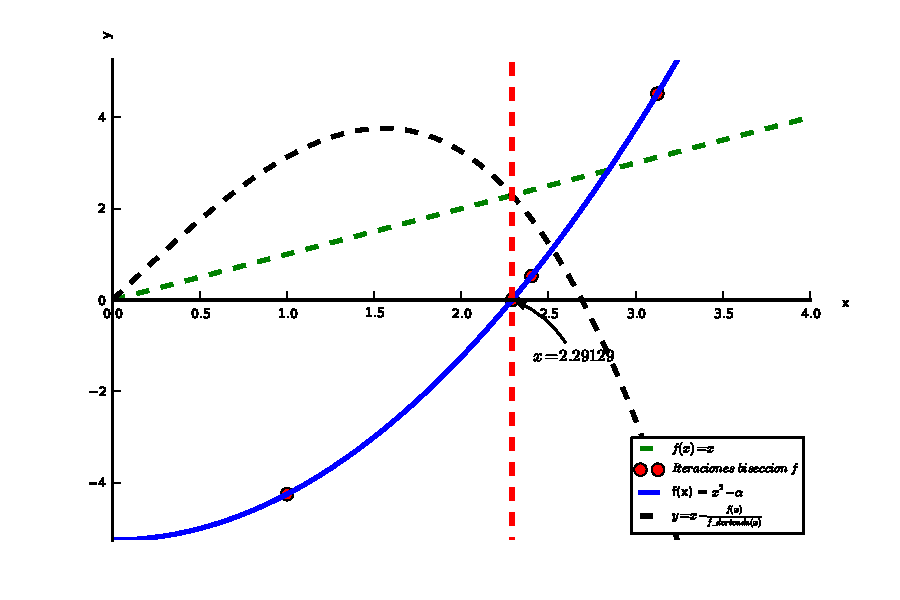
\includegraphics[keepaspectratio]{../Imagenes/exp1/newton_f.pdf}
		  \caption{newton\_f para $\alpha=5.25, \epsilon=10^{-8}, \ criterio = 5, \ seed = 1.0$}
		  \label{fig:contra1}
	\end{center}
\end{figure}
\FloatBarrier

En esta figura podemos apreciar por primera vez el comportamiento de una sucesión de punto fijo: el valor $c$ tal que $g(c)=c$ (donde $g(x) = x - \displaystyle \frac{f(x)}{f'(x)}$) es al mismo tiempo
raíz de la función $f$

Los resultados para Newton\_e, por el contrario, resultaron ser bastante distintos. Al evaluar el método para distintos valores de $\alpha$, descubrimos que: si la semilla inicial está comprendida en el intervalo
$(0,\frac{1}{\sqrt{\alpha}}]$ el método converge sin problemas. Sin embargo, empíricamente llegamos a la conclusión de que existe un $x_0$, con $x_0 > \frac{1}{\sqrt{\alpha}}$, tal que $\forall x \geq x_0$, el método
diverge si utilizamos x como semilla.

\begin{figure}[!h]
	\begin{center}
		  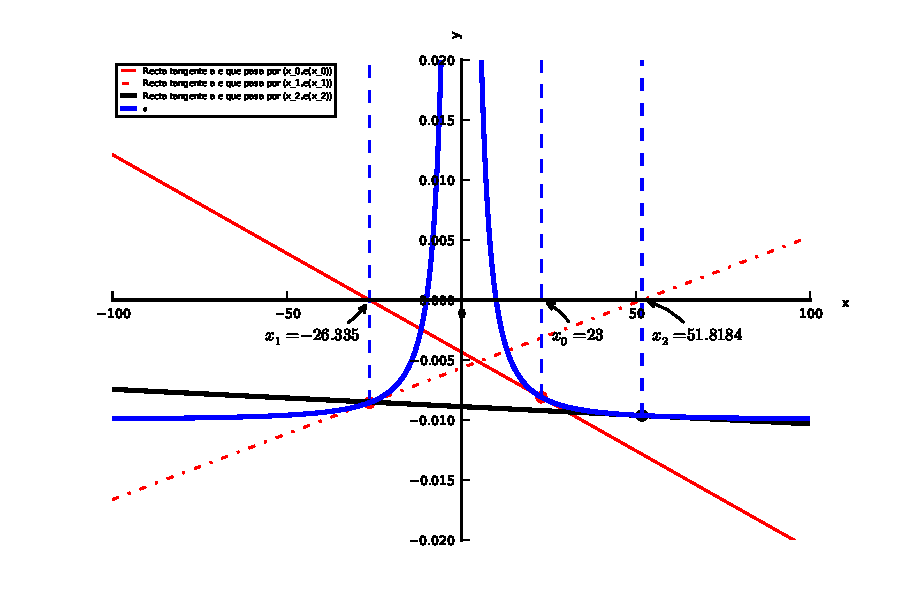
\includegraphics[keepaspectratio]{../Imagenes/exp1/divergencia.pdf}
		  \caption{Rectas tangentes a la función e con $\alpha=0.01, \frac{1}{\sqrt{\alpha}} = 10$ en $x_0= 23, x_1= -26.335, x_2=51.8184$ (primeras 3 iteraciones)}
		  \label{fig:contra1}
	\end{center}
\end{figure}
\FloatBarrier

Este gráfico nos da una idea de la causa de la divergencia para determinados valores iniciales mayores a los de la raíz buscada. La pendiente de la recta tangente en un punto está determinada por la función
e\_derivada: $\frac{-2}{x^{3}}$. Notemos que, luego de la primera iteración el valor obtenido es -26.335 $\Rightarrow$ el módulo de la pendiente de la recta tangente que pasa por $(x_1,e(x_1))$ es menor que
el anterior. Como consecuencia, la intersección de esta recta con el eje x se produce en x=51.8184, valor considerablemente más alejado del 0 que el $x_0$ inicial. De esta manera, sucesivas iteraciones 
generan puntos más distantes al 0, por lo que las pendientes de las rectas tangentes se vuelven cada vez menores en módulo, generando un círculo vicioso en donde el método diverge. Observemos cono la recta
tangente correspondiente a $(x_2,e(x_2))$, de color negro, no llega a cortar al eje x debido a su peque\~na pendiente. De hecho, esto ocurre recién en x = -617.971.

Al estudiar la convergencia de Secante\_f obtuvimos resultados bastante similares a los de Newton\_f. Empíricamente, el método converge para cualquier par de valores iniciales. Los experimentos
fueron probados para valores de $\alpha \in (0,1] \cup [1,20] \cup [1000,1010] \cup [10^{6},10^{6}+10]$, probando por cada valor distintos pares de semillas iniciales. Por ejemplo, con valores
$x_0,x_1 \in (0,1]$, $x_0 \in (0,1] \ \wedge \ x_1 \in (1,20]$, $x_0 \in (0,1] \ \wedge \ x_1 \in [1000,1010]$ , etc.

Estudiemos momentáneamente la estructura de cada iteración:

$x_{n+1} = x_n - \frac{(x_n-x_{n-1})*f(x_n)}{f(x_n)-f(x_{n-1})}$

De la fórmula se deduce que, si en algún momento $x_n = x_{n-1}$ entonces el método puede llegar a comportarse de una forma indeseada (Se realiza una división por cero, o un valor muy cercano a cero).
Por este motivo, debemos cuidarnos fundamentalmente de 2 aspectos:

a- No comenzar a iterar con semillas iniciales tales que $x_0 = x_1$.

b- Parar las iteraciones cuando $x_n \approx x_{n-1}$. En el caso de utilizar malos criterios de parada, como por ejemplo el 1: i = max\_iter
lo que sucede es que el método encuentra la raíz buscada y luego diverge, debido a que intenta continuar realizando las iteraciones.

Con Secante\_e también obtuvimos resultados similares a los de Newton\_e. El método converge con seguridad cuando $x_0,x_1 \in (0,\frac{1}{\sqrt{\alpha}}]$ Si una de las 2 semillas es mucho mayor a la raíz, lo más
probable es que el método diverja, ya que las rectas tangentes se comportan de forma muy parecida a las secantes.

~

Finalmente, para cerrar con esta primera parte, a la cual llamamos \underline{Primeras experimentaciones}, incluímos tres gráficos correspondientes a Bisección\_e, Secante\_e y Newton\_e, con el objetivo de
visualizar de forma más clara la forma en la que los métodos convergen a la raíz teórica en función de la cantidad de iteraciones. Todos ellos fueron graficados en función de los mismos datos: $\alpha = 0.01$,
criterio de parada 2 y un error $\epsilon=10^{-8}$

\begin{figure}[!h]
	\begin{center}
		  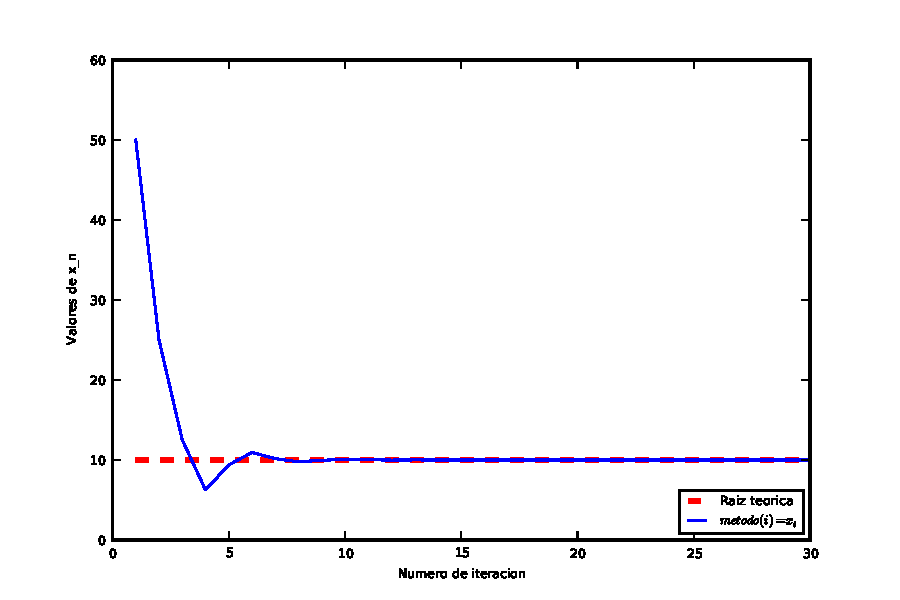
\includegraphics[keepaspectratio]{../Imagenes/exp2/biseccion_e.pdf}
		  \caption{Método de bisección\_e con los parámetros anteriormente mencionados, y semillas iniciales: $x_0 = 100, x_1=\alpha=0.01$}
		  \label{fig:contra1}
	\end{center}
\end{figure}
\FloatBarrier

Si bien en la figura anterior el método comienza con semillas bastante separadas (100 unidades aproximadamente), luego de la cuarta iteración la distancia entre ambas es solamente de 6 unidades, por lo que
alcanza el punto en donde comienzan los otros métodos. Sin embargo, realiza 30 iteraciones y aún así no llega a encontrar un resultado con un error menor al exigido: $10^{-8}$

\begin{figure}[!h]
	\begin{center}
		  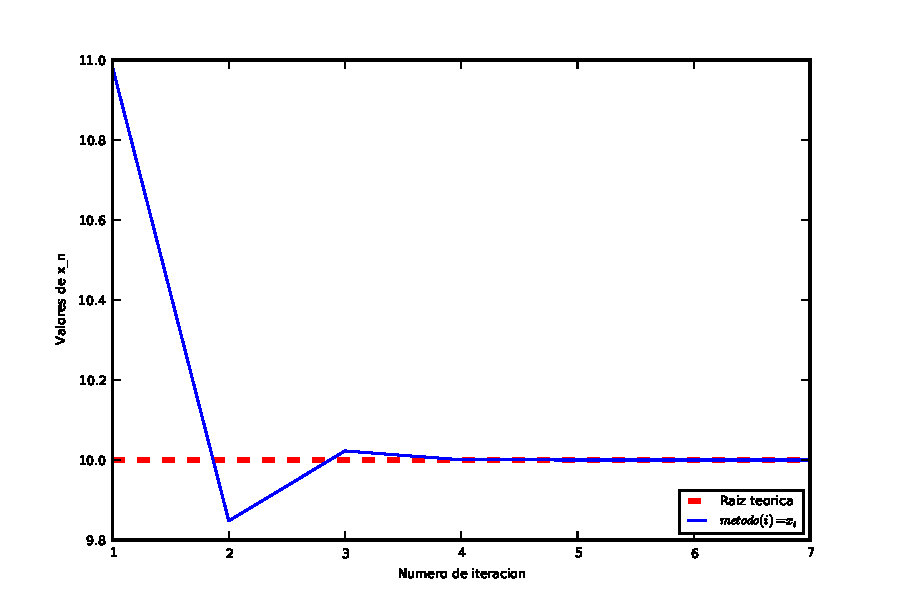
\includegraphics[keepaspectratio]{../Imagenes/exp2/secante_e.pdf}
		  \caption{Método de secante\_e con los parámetros anteriormente mencionados, y semillas iniciales: $x_0=1, x_1=11$ }
		  \label{fig:contra1}
	\end{center}
\end{figure}
\FloatBarrier

El criterio de parada se alcanza luego de la 7ma iteración en este experimento de secante\_e.

\begin{figure}[!h]
	\begin{center}
		  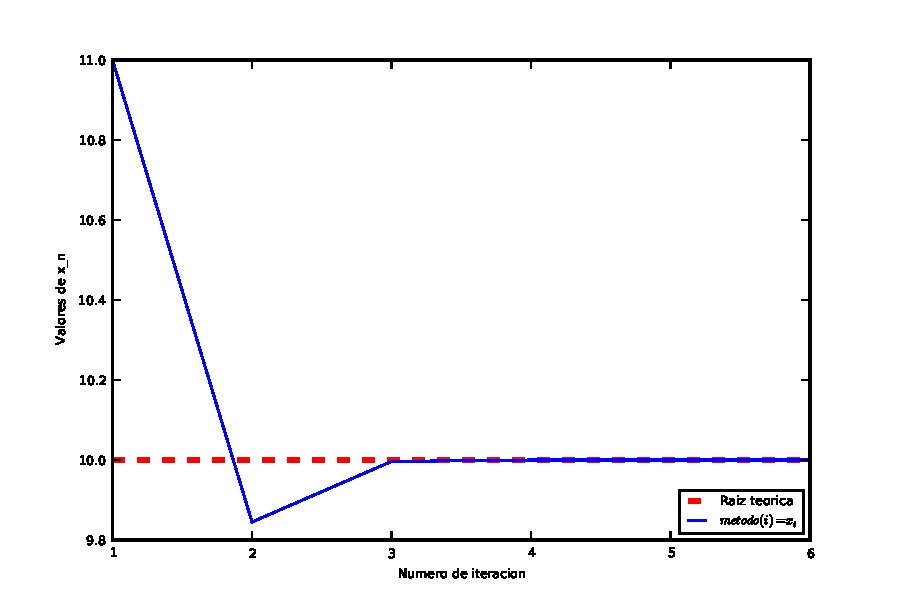
\includegraphics[keepaspectratio]{../Imagenes/exp2/newton_e.pdf}
		  \caption{Método de newton\_e con los parámetros anteriormente mencionados, y semilla inicial: $x_0=11$}
		  \label{fig:contra1}
	\end{center}
\end{figure}
\FloatBarrier

El criterio de parada se alcanza luego de la 6ta iteración en este experimento de Newton\_e.

\begin{figure}[!h]
	\begin{center}
		  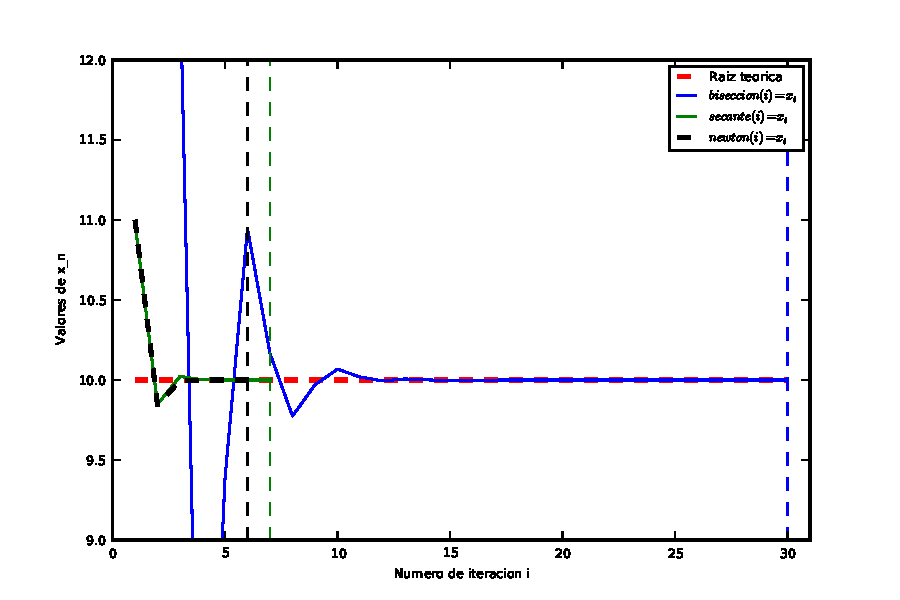
\includegraphics[keepaspectratio]{../Imagenes/exp2/todos_juntos.pdf}
		  \caption{Todos juntos en un mismo gráfico}
		  \label{fig:contra1}
	\end{center}
\end{figure}
\FloatBarrier

\subsection{Fijando criterios de parada}

Probamos los 5 criterios para la función $f$ y los siguientes métodos, con distintos valores de $\alpha$ y de $\epsilon$. En todos los casos el comportamiento fue similar, por lo que
seleccionamos una instancia particular: $\alpha = 901$ y $\epsilon=10^{-10}$ para ser analizada.

\begin{center}
    \small{
    \begin{tabular}{| l | l | l | l | l | l | l | l | l | l | l | l | l |}
    \hline
    Métodos & c2/dif & c2/iter & c3/dif & c3/iter & c4/dif & c4/iter & c5/dif & c5/iter & c6/dif & c6/iter \\ \hline
    Biseccion\_f & $4*10^{-11}$ & 44 & $2*10^{-9}$ & 39 & $2*10^{-12}$ & 47 & $3*10{-13}$ & 49 & 0 & max\\ \hline
    Newton\_f & 0 & 11 & 0 & 11 & $9*10{-14}$ & 10 & 0 & 11 & 0 & max \\ \hline
    Secante\_e & 0 & 15 & 0 & 14 & 0 & 14 & 0 & 15 & nan & max \\ \hline
    \end{tabular}
    }
\end{center}

La tabla muestra por cada método y por cada uno de los distintos criterios de parada
la diferencia entre el resultado obtenido y la raíz teórica (calculada con la función $sqrt$ de c++), y la cantidad de iteraciones antes de la finalización del método debido a dicho criterio.
Al contrastar los resultados obtenidos con nuestras hipótesis previas (planteadas en el desarrollo) no obtuvimos grandes diferencias. Tal como suponíamos, el criterio 4) $|f(x_{n})| < \epsilon$ funciona
de forma correcta (levemente mejor que el 2) y el 3) ). Queda demostrado que el 5) es también un buen criterio. Donde si nos llevamos una sorpresa fue en el comportamiento del 6). Sin embargo, entender lo
que sucede resulta bastante intuitivo. A medida que el método va convergiendo, el denominador se acerca a cero tan rápidamente como lo hace el numerador, por lo que la cota establecida por el criterio
nunca se alcanza y el método itera la cantidad máxima de iteraciones. Esto es particularmente malo en secante, ya que hace que el método diverja.

También realizamos experimentos similares para la función $e$, entre los cuales seleccionamos 2 posibles escenarios: Uno con un valor de $\alpha$ muy peque\~no y otro en donde es mayor. La primera tabla
está construída con valores obtenidos al correr los métodos con $\alpha=10 \ , \epsilon = 10^{-10}$. Para el caso de Newton, la semilla inicial fue $\frac{1}{\alpha} = 0.1$.
Para el caso de Secante las semillas iniciales fueron $0.1$ y $0.5$.
\begin{center}
    \small{
    \begin{tabular}{| l | l | l | l | l | l | l | l | l | l | l | l | l |}
    \hline
    Métodos & c2/dif & c2/iter & c3/dif & c3/iter & c4/dif & c4/iter & c5/dif & c5/iter & c6/dif & c6/iter \\ \hline
    Biseccion\_e & $6*10^{-11}$ & 37 & $6*10^{-12}$ & 39 & $9*10^{-13}$ & 41 & $3*10^{-13}$ & 43 & $6*10^{-17}$ & 60 \\ \hline
    Newton\_e & 0 & 9 & 0 & 10 & 0 & 9 & 0 & 10 & 0 & max \\ \hline
    Secante\_e & 0 & 12 & 0 & 12 & $3*10^{-14}$ & 11 & 0 & 12 & nan & max \\ \hline
    \end{tabular}
    }
\end{center}

Los resultados obtenidos fueron muy similares a los del experimento anterior. Los criterios 4) y 5) (relacionados con las imágenes) se comportan de forma correcta, al igual que 2) y 3) (relacionados con los
términos de la sucesión). El criterio 6) vuelve a fallar al tener un denominador muy peque\~no, por lo que los métodos nunca frenan (salvo en el caso de bisección)
y realizan la cantidad máxima de iteraciones. Al igual que en $f$, esto hace que secante diverja.

Finalmente realizamos un test para la función $e$ con $\alpha = 10^{-8}$ y $\epsilon = 10^{-5}$. Las semilla inicial para Newton\_e fue $x_{0}=1$. Las semillas iniciales para Secante\_e fueron $x_{0} = 0.1$, 
$x_{1} = 0.5$

\begin{center}
    \small{
    \begin{tabular}{| l | l | l | l | l | l | l | l | l | l | l | l | l |}
    \hline
    Métodos & c2/dif & c2/iter & c3/dif & c3/iter & c4/dif & c4/iter & c5/dif & c5/iter & c6/dif & c6/iter \\ \hline
    Biseccion\_e & $4*10^{-6}$ & 44 & $8*10^{-2}$ & 30 & \textcolor{red}{$5*10^{7}$} & \textcolor{red}{1} & \textcolor{red}{$2.5*10^{7}$} & \textcolor{red}{2} & {$2.5*10^{7}$} & 2  \\ \hline
    Newton\_e & 0 & 28 & $6.1*10^{-7}$ & 27 & \textcolor{red}{$10^{4}$} & \textcolor{red}{15} & \textcolor{red}{$10^{4}$} & \textcolor{red}{15} & 0 & max \\ \hline
    Secante\_e & 0 & 44 & $1.5*10^{-7}$ & 43 & \textcolor{red}{$10^{4}$} & \textcolor{red}{25} & \textcolor{red}{$10^{4}$} & \textcolor{red}{24} & nan & max   \\ \hline
    \end{tabular}
    }
\end{center}

Los resultados concuerdan con nuestras hipótesis iniciales. La pendiente de la recta tangente a la función $e$ para x tales que $x >> 0$ es muy peque\~na, por lo que 4) y 5) no constituyen buenos
criterios de parada. Para casos en donde $\alpha$ es muy peque\~no es conveniente utilizar 2) y 3), ya que no dependen del valor de las imágenes.

\subsection{Estableciendo una buena semilla}





